\documentclass[11pt,a4paper,headsepline]{scrartcl}
\usepackage[utf8]{inputenc}
\usepackage[german]{babel}
\usepackage{amsmath}
\usepackage{amsfonts}
\usepackage{amssymb}
\usepackage{tikz}
\usepackage[left=2cm,right=2cm,top=2cm,bottom=2cm]{geometry}
\usepackage[utf8]{inputenc}
\usepackage{graphicx}
\usepackage{pgfplots}
\usepackage{fancyhdr}
\usepackage[scaled]{helvet}
\usepackage{paralist}
\usepackage{pdfpages}

\usetikzlibrary{calc}
\newtheorem{aufgabe}{Aufgabe}

\renewcommand*\familydefault{\sfdefault}
\renewcommand{\arraystretch}{1.1}

\title{\"Ubung Kraftschluss-Schlupf}
\date{}
\makeatletter
\let\Title\@title
\let\Author\@author
\makeatother
\pagestyle{fancy}
\fancyhead[L]{Prof. Dr. Raphael Pfaff}
\fancyhead[R]{84111: Schienenfahrzeugtechnik}
\fancyfoot[L]{Datei: \jobname}
\fancyfoot[R]{Datum: \today \vspace{.1cm}
\begin{picture}(0,0)(0,0)\put(.5,1){
\includegraphics[height=5cm]{fh_logo}}\end{picture}}

\begin{document}
\maketitle
\thispagestyle{fancy}
\pagestyle{fancy}
\vspace{-2cm}

\begin{aufgabe}[Kraftschlussausnutzung]
Ein dreiteiliger Triebzug wird beschleunigt und gebremst. Die Daten des Triebzugs sind:
\begin{itemize}
	\item Achsformel Bo' Bo' + 2' 2' + Bo' Bo'
	\item $m_{W,i} = 40 \mathrm{t}$
	\item Massenfaktoren (anteilig von $m_{W,i}$):
	\begin{itemize}
		\item Treibachsen $\rho_{T} = 1{,}15$
		\item Laufachsen $\rho_{L} = 1{,}08$
	\end{itemize} 
	\item Beschleunigungsverm\"ogen: $a_{max} = 1{,}5 \frac{\mathrm{m}}{\mathrm{s}^2}$
	\item Verz\"ogerung der Schnellbremse: $b_{max} = 1{,}2 \frac{\mathrm{m}}{\mathrm{s}^2}$
\end{itemize} 

Bestimmen Sie:
\begin{enumerate}[a)]
\item Treibachsbremskr\"afte (Lauf- und Treibachsen) und Kraftschlussausnutzung w\"ahrend einer Schnellbremsung
\item Treibachszugkraft und Kraftschlussausnutzung w\"ahrend der maximalen Beschleunigung
\item \label{Ta:FrictionCoeff} Die Bremse muss an zwei Drehgestellen (1 Laufdrehgestell, 1 Triebdrehgestell) auf Grund eines Fehlers abgesperrt werden. Bestimmen Sie die verbleibende Verz\"ogerung sowie die Kraftschlussausnutzung, f\"ur die die Bremsleistung konstant gehalten werden k\"onnte. Lassen sich die Grenzwerte der TSI Loc \& Pas einhalten?
\item \label{Ta:Stochastisch}Der Rad-Schiene-Kraftschluss sei wie in Abbildung \ref{Fig:Stochastisch} statistisch zu modellieren. Markieren Sie den in Aufgabe \ref{Ta:FrictionCoeff} ermittelten Reibwert. Schraffieren Sie den Bereich, der die Wahrscheinlichkeit des Schleuderns angibt.
		\begin{figure}[htbp]
                        \begin{center}
                        \begin{tikzpicture}[baseline] \begin{axis}[
                        	width = 12cm, height = 7cm,
                           %title=Inv. cum. normal,
                           xlabel={$\mu_{R/S}$},
                           ylabel={$p$},
                           xmin=0, xmax=0.5,
                        	 grid = major, 
	 		 yticklabels = {,,},
                           %minor y tick num=1,
                        ]
                                          
                        \newcommand\MU{.25}
                        \newcommand\SIGMA{0.065}
                        \addplot[blue,domain=0:0.5,samples=201]
                           {exp(-(x-\MU)^2 / 2 / \SIGMA^2) / (\SIGMA * sqrt(2*pi))};
                        \end{axis}
                        \end{tikzpicture}
                        \caption{Wahrscheinlichkeitsdichte des Reibwerts zu Aufgabe \ref{Ta:Stochastisch}}
                        \label{Fig:Stochastisch}
                        \end{center}
                    \end{figure}
\end{enumerate}
\end{aufgabe}
\vspace{0.5cm}
\begin{aufgabe}
Ein G\"uterwagen (Masse leer $m_{L} = 30 \mathrm{t}$, Masse unter maximaler Beladung $m_{B} = 80 \mathrm{t}$, rotierende Masse $m_{R} = 3{,}2 \mathrm{t}$) erreicht eine maximale Verz\"ogerung $b_{max} = 0{,}7 \frac{\mathrm{m}}{\mathrm{s}^2}$.
Bestimmen Sie:
\begin{enumerate}[a)]
\item Treibachsbremskraft und Kraftschlussausnutzung w\"ahrend einer Schnellbremsung des beladenen Wagens
\item Kraftschlussausnutzung w\"ahrend einer Schnellbremsung des unbeladenen Wagens unter der Annahme einer konstanten Bremskraft am Radumfang
\item Treibachsbremskraft des unbeladenen Wages f\"ur eine Kraftschlussausnutzung von $0{,1}$.
\end{enumerate}
\end{aufgabe}
\newpage
%\subsection*{Auszug TSI Loc \& Pas}
 \includepdf[scale = 0.9,turn = false, pages = {48-49}, pagecommand ={\pagestyle{fancy}}]{TSILocPas.pdf}
\end{document}